% Copyright 2016 - 2018 Bas van Meerten and Wouter Franssen
%
%This file is part of ssNake.
%
%ssNake is free software: you can redistribute it and/or modify
%it under the terms of the GNU General Public License as published by
%the Free Software Foundation, either version 3 of the License, or
%(at your option) any later version.
%
%ssNake is distributed in the hope that it will be useful,
%but WITHOUT ANY WARRANTY; without even the implied warranty of
%MERCHANTABILITY or FITNESS FOR A PARTICULAR PURPOSE.  See the
%GNU General Public License for more details.
%
%You should have received a copy of the GNU General Public License
%along with ssNake. If not, see <http://www.gnu.org/licenses/>.

\documentclass[11pt,a4paper]{article}
% Copyright 2016 - 2017 Bas van Meerten and Wouter Franssen
%
%This file is part of ssNake.
%
%ssNake is free software: you can redistribute it and/or modify
%it under the terms of the GNU General Public License as published by
%the Free Software Foundation, either version 3 of the License, or
%(at your option) any later version.
%
%ssNake is distributed in the hope that it will be useful,
%but WITHOUT ANY WARRANTY; without even the implied warranty of
%MERCHANTABILITY or FITNESS FOR A PARTICULAR PURPOSE.  See the
%GNU General Public License for more details.
%
%You should have received a copy of the GNU General Public License
%along with ssNake. If not, see <http://www.gnu.org/licenses/>.

\usepackage[british]{babel}
\usepackage{graphicx,booktabs,listings,amsmath,pgfplots,pgfplotstable}
\usepackage[small,bf,nooneline]{caption}
\usepackage{subcaption}
\usepackage[sort&compress,numbers]{natbib}
\usepackage{tikz}
\usepackage{mathtools}
\usepackage[nottoc]{tocbibind}%adds bibliography to table of contents.
\graphicspath{{./images/}}
%\setlength{\textwidth}{453pt} %597 pt is the a4 paperwidth. Minus 2 in margin. 72 pt = 1 in
%\setlength{\hoffset}{-\oddsidemargin}
%\setlength{\voffset}{-30pt} %
%\setlength{\textheight}{651 pt} %a4 height 845 pt minus 2* total headheight. In this case 2*88pt
%% examine margines via the layout package. Use command \layout{} in document to draw a picture.
%\setlength{\parindent}{0.5 cm}
%\setlength{\parskip}{0 cm}
\usepackage[left=82pt,right=82pt,top=95pt,bottom=95pt,footnotesep=0.5cm]{geometry}
%\setlength{\headheight}{14pt}

%define colours--------------------
%dark
\usepackage{xcolor}
\definecolor{MyGrayD}{RGB}{1,1,1}
\definecolor{MyRedD}{RGB}{237,45,46}
\definecolor{MyGreenD}{RGB}{0,140,71}
\definecolor{MyBlueD}{RGB}{24,89,169}
\definecolor{MyOrangeD}{RGB}{243,125,34}
\definecolor{MyPurpleD}{RGB}{102,44,145}
\definecolor{MyBrownD}{RGB}{161,29,32}
\definecolor{MyPinkD}{RGB}{179,56,147}
%normal
\definecolor{MyGray}{RGB}{114,114,114}
\definecolor{MyRed}{RGB}{241,89,95}
\definecolor{MyGreen}{RGB}{121,195,106}
\definecolor{MyBlue}{RGB}{89,154,211}
\definecolor{MyOrange}{RGB}{249,166,90}
\definecolor{MyPurple}{RGB}{158,102,171}
\definecolor{MyBrown}{RGB}{205,112,88}
\definecolor{MyPink}{RGB}{215,127,179}
%light
\definecolor{MyGrayL}{RGB}{204,204,204}
\definecolor{MyRedL}{RGB}{242,174,172}
\definecolor{MyGreenL}{RGB}{216,228,170}
\definecolor{MyBlueL}{RGB}{184,210,235}
\definecolor{MyOrangeL}{RGB}{242,209,176}
\definecolor{MyPurpleL}{RGB}{212,178,211}
\definecolor{MyBrownL}{RGB}{221,184,169}
\definecolor{MyPinkL}{RGB}{235,191,217}
%----------------------------------

%Figure ref with hyperref
\newcommand{\fref}[1]{\hyperref[#1]{Figure \ref*{#1}}}
\newcommand{\sref}[1]{\hyperref[#1]{Section \ref*{#1}}}
\newcommand{\tref}[1]{\hyperref[#1]{Table \ref*{#1}}}

%Makes a new command for figures with input values: filename, width(times linewidth),
% caption and label.
\newcommand{\onefigure}[4]{
\setlength{\captionwidth}{#2\linewidth}
\begin{figure}
\includegraphics[width=#2\linewidth]{#1}
\centering
\parbox{\linewidth}{\caption{#3}
\label{#4}}
\end{figure}
}

%Makes a new command for tikz figures with input values: tikz commands, 
% caption and label.
\newcommand{\onetikz}[3]{
\settowidth{\captionwidth}{#1}
\ifthenelse{\lengthtest{\captionwidth<0.7\linewidth}}{\setlength{\captionwidth}{0.7\linewidth}}{}

\begin{figure}
\centering
#1
\centering
\parbox{\linewidth}{\caption{#2}
\label{#3}}
\end{figure}
}

%Makes a new command for two figures next to each other with input values: filename1, caption1, label1,filename2, caption2 and label2. Figure width is set to 0.47\linewidth and the space between the figures is filled with \hfill so the sides of the figures align with to edge of the line.
\newcommand{\twofigure}[6]{
\setlength{\captionwidth}{\linewidth}
\begin{figure*}[ht!]
\begin{minipage}[t]{0.47\linewidth}
\includegraphics[width=\linewidth]{#1}
\centering
\caption{#2}
\label{#3}
\end{minipage}
\hfill
\begin{minipage}[t]{0.47\linewidth}
\centering
\includegraphics[width= \linewidth]{#4}
\centering
\caption{#5}
\label{#6}
\end{minipage}
\end{figure*}
}


%Makes a new command for a table with caption witdh equal to the total table width. Input: tabular, caption and label. Example:
%\onetable{
%\begin{tabular}{ccc}
%a&b&c\\
%\hline
%1&1&1\\
%1&1&1\\
%1&1&1\\
%\end{tabular}
%{The caption.}
%{tab:table1}
%}
\newcommand{\onetable}[3]{
\settowidth{\captionwidth}{#1}
\ifthenelse{\lengthtest{\captionwidth<0.7\linewidth}}{\setlength{\captionwidth}{0.7\linewidth}}{}
\begin{table}
\caption{#2}
\vspace{-0.24cm} %Puts caption close to toprule
\label{#3}
\centering
#1
\end{table}
}

%Makes a long table with captionwidth equal to tablewidth. It takes the following arguments:
%1: Column specifier (e.g. cccc)
%2: Caption
%3: Label
%4: First head (i.e. first row of regular table)
%5: Head of consecutive pages
%6: Foot of pagebreak
%7: Lastfoot (e.g. \midrule)
%8: Body of table
\newcommand{\onelongtable}[8]{
\begin{center}
\settowidth{\captionwidth}{
\begin{tabular}{#1}
#4
#8
\end{tabular}} % This ends the captionwidth part. Next comes the real table.

\begin{longtable}{#1}
\caption{#2}\\
\vspace{-0.74cm} %Puts caption close to toprule
\label{#3}\\

#4
\endfirsthead

#5
\endhead

#6
\endfoot

#7
\endlastfoot

#8
\end{longtable}
\end{center}}




%1:pgfplots code
%2:width
%3:caption
%4:label
\newcommand{\pgfplotsfigure}[4]{
\pgfplotsset{width=#2\linewidth}
\setlength{\captionwidth}{#2\linewidth}
\begin{figure}[t]
\centering
#1
\centering
\parbox{\linewidth}{\caption{#3}
\label{#4}}
\end{figure}
}


\usepackage[bitstream-charter]{mathdesign}
\usepackage[T1]{fontenc}
\usepackage[protrusion=true,expansion,tracking=true]{microtype}
\pgfplotsset{compat=1.7,/pgf/number format/1000 sep={}, axis lines*=left,axis line style={gray},every outer x axis line/.append style={-stealth'},every outer y axis line/.append style={-stealth'},tick label style={font=\small},label style={font=\small},legend style={font=\footnotesize}}
\usepackage{colortbl}
\usetikzlibrary{calc}

%Set section font
\usepackage{sectsty}
\allsectionsfont{\color{black!70}\fontfamily{SourceSansPro-LF}\selectfont}
%--------------------


%Set toc fonts
\usepackage{tocloft}
%\renewcommand\cftchapfont{\fontfamily{SourceSansPro-LF}\bfseries}
\renewcommand\cfttoctitlefont{\color{black!70}\Huge\fontfamily{SourceSansPro-LF}\bfseries}
\renewcommand\cftsecfont{\fontfamily{SourceSansPro-LF}\selectfont}
%\renewcommand\cftchappagefont{\fontfamily{SourceSansPro-LF}\bfseries}
\renewcommand\cftsecpagefont{\fontfamily{SourceSansPro-LF}\selectfont}
\renewcommand\cftsubsecfont{\fontfamily{SourceSansPro-LF}\selectfont}
\renewcommand\cftsubsecpagefont{\fontfamily{SourceSansPro-LF}\selectfont}
%--------------------

%Define header/foot
%\usepackage{fancyhdr}
%\pagestyle{fancy}
%\fancyhead[LE,RO]{\fontfamily{SourceSansPro-LF}\selectfont \thepage}
%\fancyhead[LO,RE]{\fontfamily{SourceSansPro-LF}\selectfont \leftmark}
%\fancyfoot[C]{}
%--------------------

%remove page number from first chapter page
%\makeatletter
%\let\ps@plain\ps@empty
%\makeatother
%----------------------

\usepackage[hidelinks,colorlinks,allcolors=black, pdftitle={MQMAS processing in ssNake},pdfauthor={Wouter M.J.\ Franssen}]{hyperref}

\interfootnotelinepenalty=10000 %prevents splitting of footnote over multiple pages
\linespread{1.2}

\title{\color{black}\fontfamily{SourceSansPro-LF}\bfseries REDOR processing in ssNake}
\author{}
\date{\color{black}\fontfamily{SourceSansPro-LF}\bfseries \today}


\begin{document}
%\newgeometry{left=72pt,right=72pt,top=95pt,bottom=95pt,footnotesep=0.5cm}
\microtypesetup{protrusion=true} % enables protrusion

\maketitle

\section{Introduction}
The following will explain how rotational-echo double-resonance (REDOR) NMR data can be processed in ssNake.
 The
tutorial delivered with the ssNake program is considered as prior knowledge. If you have not yet
studied this, please do so before continuing with this example.

In a REDOR experiment, echo spectra are recorded with an increase in echo time $\tau$. As the
experiment is recorded in spinning fashion, the echo time must be multiple of the rotor period
$1/\nu_\text{r}$. In the experiment, the spinning cause the dipolar couplings to be less effective.
The goal of a REDOR experiment is to get information on the dipolar couplings between two nuclei of
a different type, while still having the resolution enhancing MAS active. This is done by performing
the echo experiments twice: once as is, and other time using 180 degree pulses on the other nuclei.
The goal of these pulses is to reintroduce (recouple) the dipolar coupling, causing a strong dephasing during
the echo time. Essentially, this is a measure of the effective $T_2^*$ polarization loss in the
presence or absence of the dipolar coupling.

Measuring REDOR data leads to two data sets: one with, and one without the recoupling pulses. Both
these data sets are an array of 1D spectra, for increasing echo times (number of rotor periods). For
each echo time, we determine the integral (or peak height) of a peak. We get two integrals of the relevant peak: without pulse ($S_\text{wo}$) and with
pulses ($S_\text{wi}$). The relevant information we need, is the relative difference between these:
\begin{equation*}
  \Delta S = \frac{S_\text{wo} - S_\text{wi}}{S_\text{wo}}
\end{equation*}
A REDOR plot feature this $\Delta S$ as a function of echo time (or rotor periods).





\section{Data}
The data in this tutorial was recorded on a Varian 400 MHz machine on glycine using 5 kHz MAS. The
data were recorded with 2 to 40 rotor periods per echo delay (with steps of 2).



\section{Processing}
Processing REDOR data is not that hard. Only a couple of steps are needed.

\begin{itemize}
	\item Open the REDOR\_no\_pulse.fid data using File $\longrightarrow$ Open
	\item Zerofill to 16384 points (Matrix  $\longrightarrow$ Sizing)
	\item Fourier Transform
	\item Phase with $-6.0$ degrees 0 order phasing (Tools $\longrightarrow$ Phasing)
\end{itemize}
This gives the following:
\begin{center}
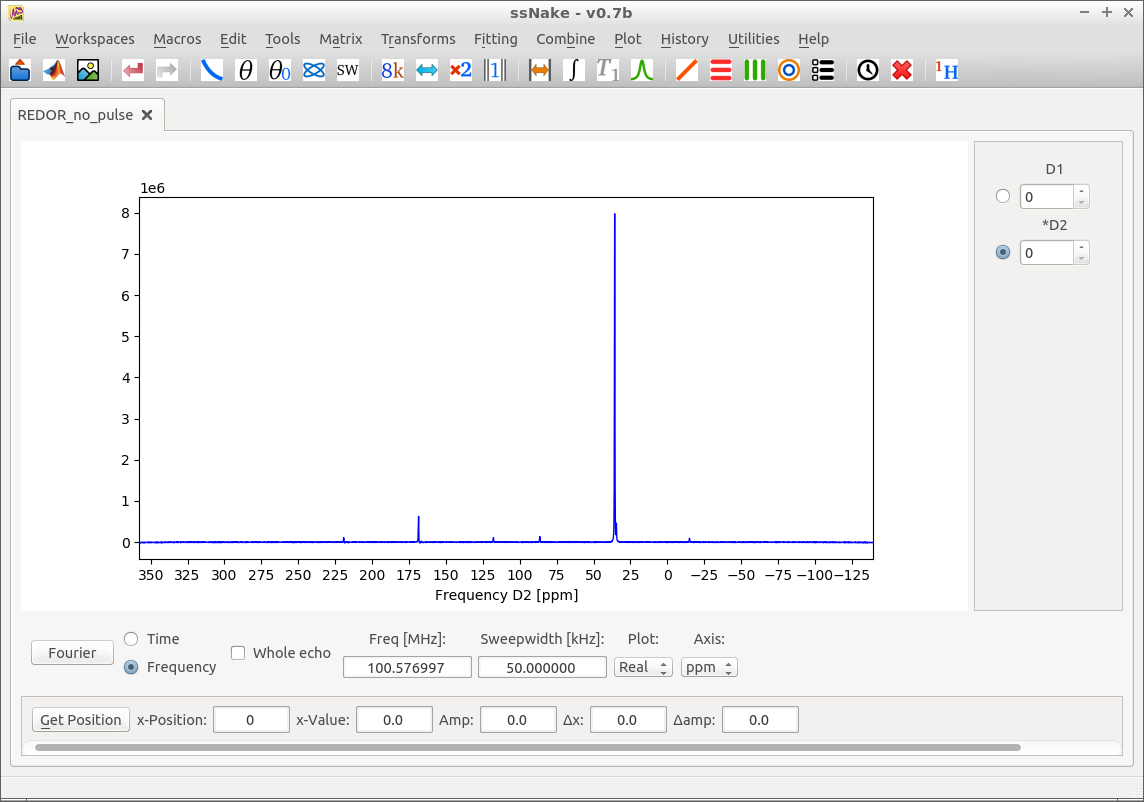
\includegraphics[width=0.8\linewidth]{Figs/Fig1.png}
\end{center}
In this case, we are interested in the right peak (CH$_2$). We want a plot of the integral of this
line over all the 11 spectra. For this, we integrate the peak. Note that ssNake has two types of
integral: via Fitting  $\longrightarrow$ Integrals, which can be seen as a way to ask ssNake
`what is the integral of this peak'. Or via Matrix $\longrightarrow$ Region $\longrightarrow$
Integrate, which integrates a region across all traces and changes the data to lose the integrated
dimension. In this case, we need the latter.

\begin{itemize}
	\item Use Matrix $\longrightarrow$ Region $\longrightarrow$
Integrate and click on the left and right side of the CH2 peak (ignore the tiny peak next to it for
the moment). In my case, these are positions 5679 and 5861.
\end{itemize}
This should give:
\begin{center}
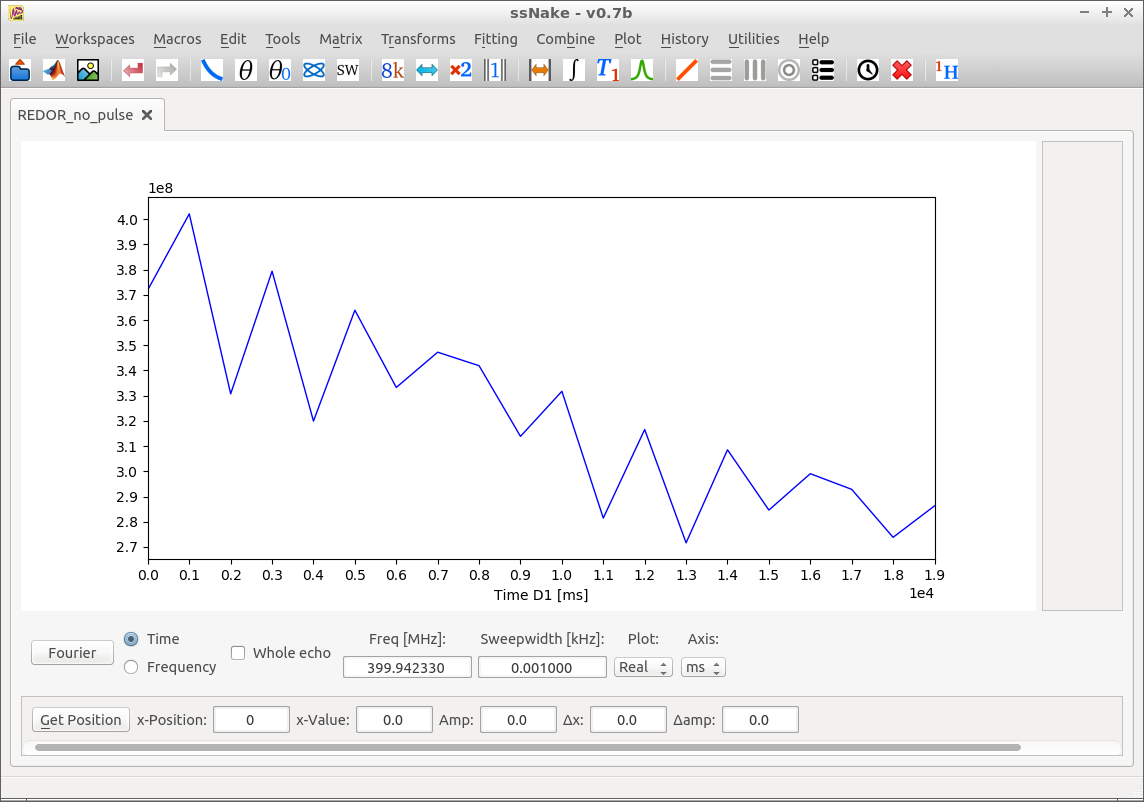
\includegraphics[width=0.8\linewidth]{Figs/Fig2.png}
\end{center}
This shows how the integral decays in the experiment without the pulses (dipolar coupling disabled).

Now, we need to do the same for the data with the pulses. 
\begin{itemize}
	\item Open the REDOR\_with\_pulse.fid data using File $\longrightarrow$ Open
\end{itemize}
Do the same processing as for the other data, but now with $-5.0$ degrees phasing. After
integrating, this should give:
\begin{center}
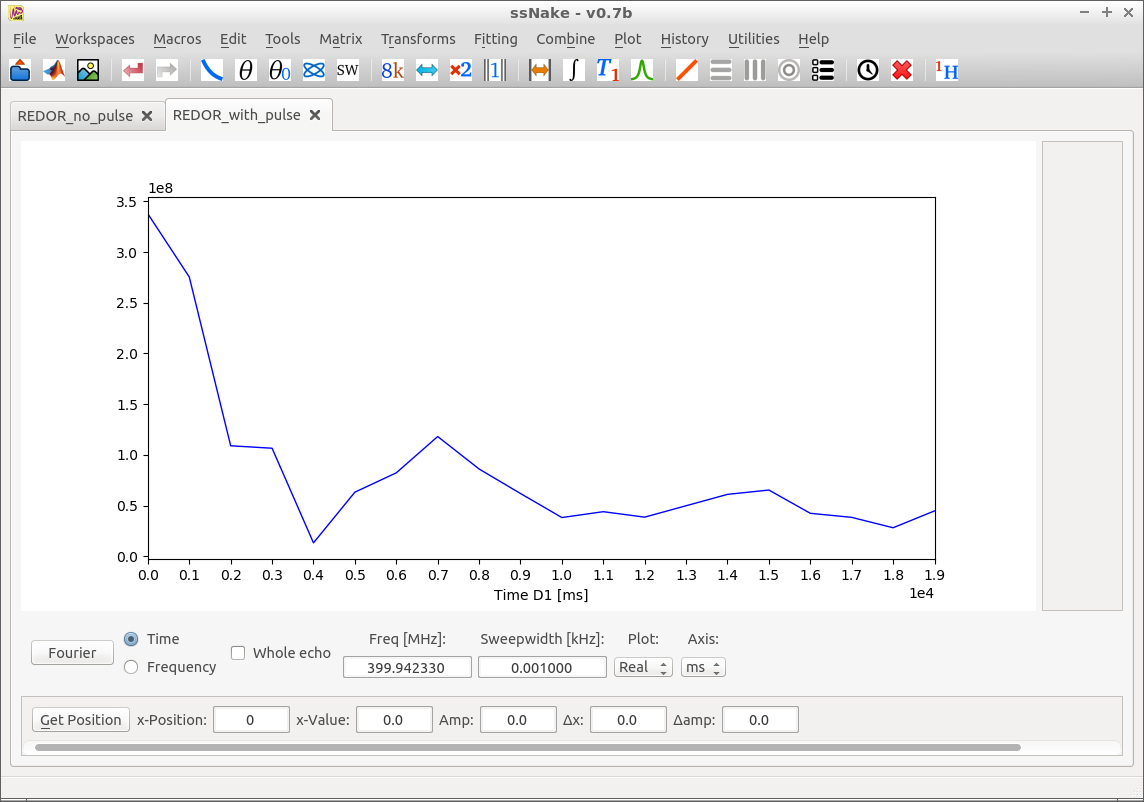
\includegraphics[width=0.8\linewidth]{Figs/Fig3.png}
\end{center}
Now, there are multiple ways to continue, either you can export both data sets via File
$\longrightarrow$ Export  $\longrightarrow$ ASCII, and do further processing in your favourite
software, or we can continue within ssNake. Just for the sake of it, we will continue in ssNake.

We want a plot of:
\begin{equation*}
  \Delta S = \frac{S_\text{wo} - S_\text{wi}}{S_\text{wo}}
\end{equation*}
for each point. To do this, we make a copy of the no\_pulse data set:
\begin{itemize}
	\item When on the `REDOR\_no\_pulse' data, use Workspaces $\longrightarrow$ Duplicate (and name
	  it `Diff').
\end{itemize}
Now, we must subtract the data with the pulses. While in the `Diff' workspace:
\begin{itemize}
	\item Combine $\longrightarrow$ Subtract (and select the `REDOR\_with\_pulse' data)
\end{itemize}
This should give:
\begin{center}
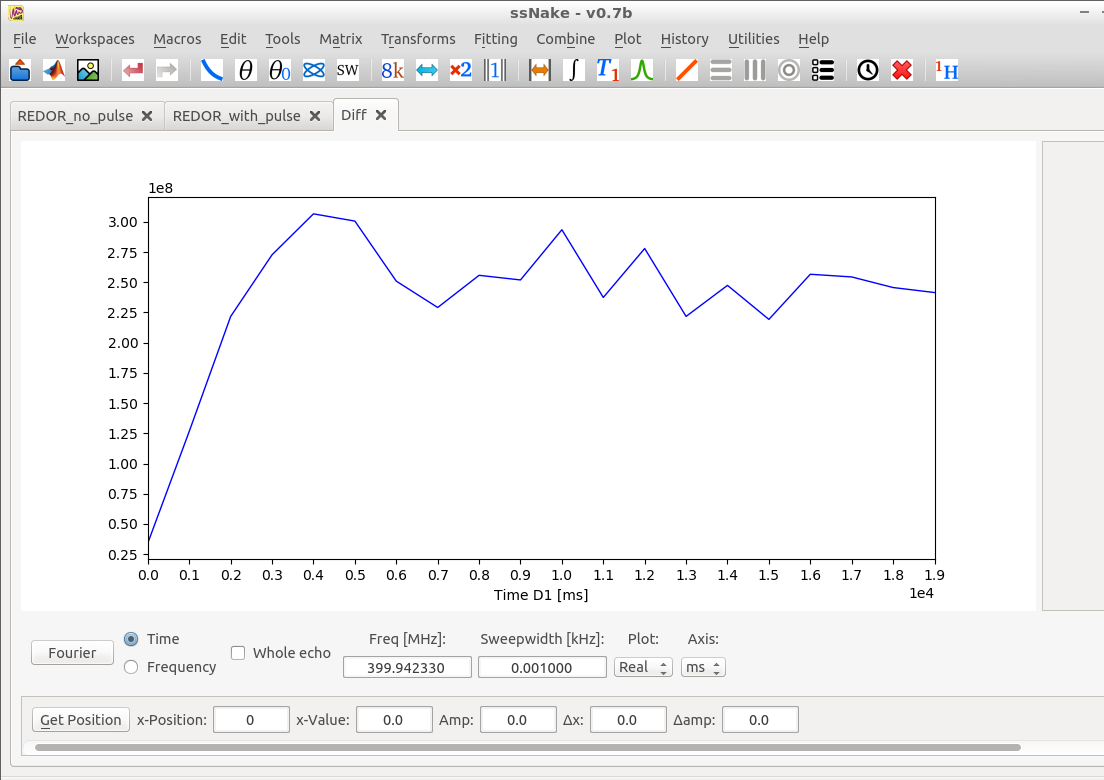
\includegraphics[width=0.8\linewidth]{Figs/Fig4.png}
\end{center}
Now, we must divide the data by $S_\text{wo}$. However, we must realize that, when dividing data, we
do not want to do a complex divide (we have complex numbers). Therefore, we must first take the real
values of the data:
\begin{itemize}
	\item In workspace `Diff' do Tools $\longrightarrow$ Real
	\item In workspace `REDOR\_no\_pulse' do Tools $\longrightarrow$ Real
	\item In workspace `Diff' do  Combine $\longrightarrow$ Divide, and select `REDOR\_no\_pulse'
\end{itemize}
This gives:
\begin{center}
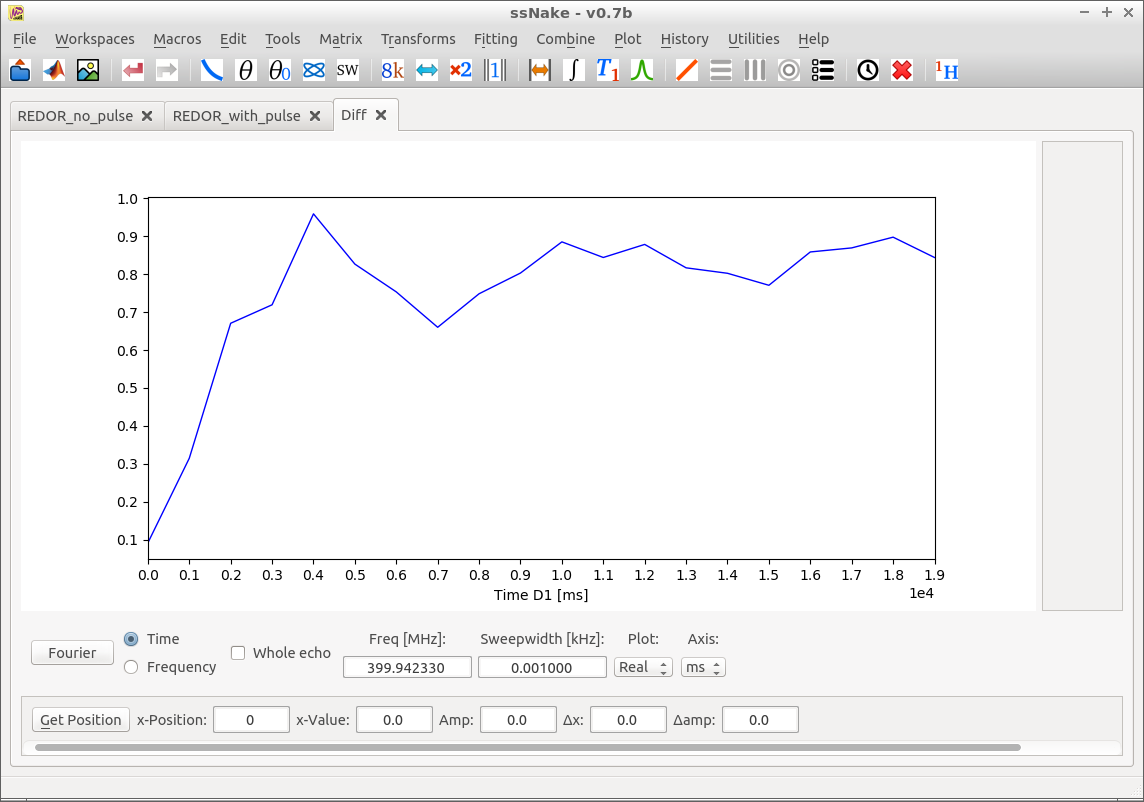
\includegraphics[width=0.8\linewidth]{Figs/Fig5.png}
\end{center}
Which is clearly between 0 and 1 (as it should be).

Now, we can set the axis. The first point was 2 rotor periods, the last 40. Note that this means 4
and 80 for the total echo time. The spinning speed was 5 kHz, so a period is 0.2 ms. This measn that
the axis should go from 0.8 to 32 ms:
\begin{itemize}
	\item In workspace `Diff' use Plot $\longrightarrow$ User X-axis (Type: Linear, Start: 0.8e-3,
	  Stop: 32e-3)
\end{itemize}
This gives the final figure:
\begin{center}
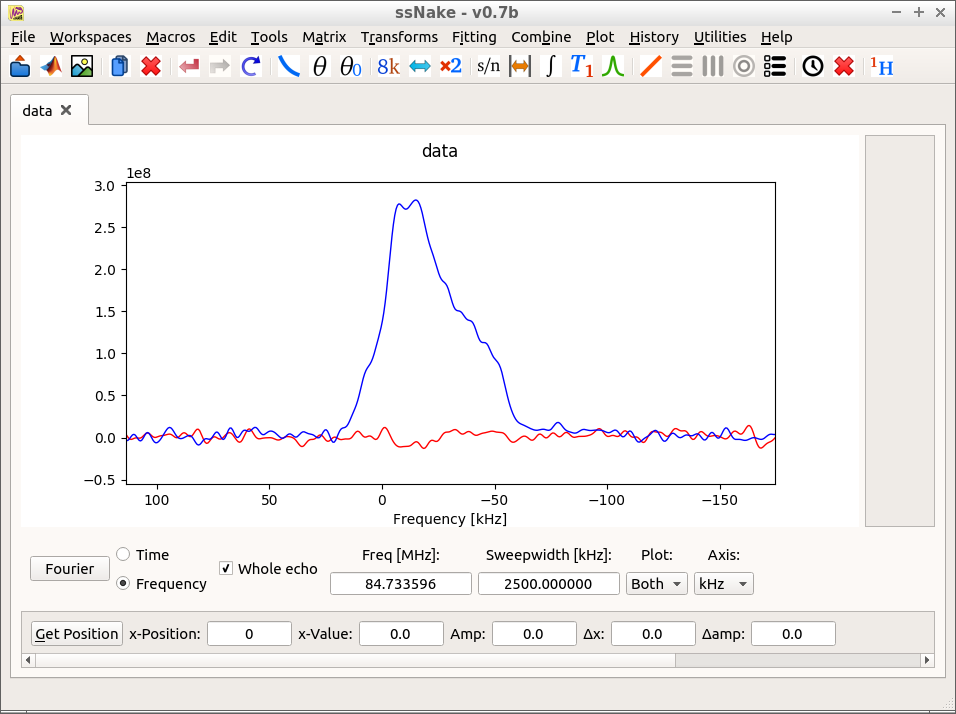
\includegraphics[width=0.8\linewidth]{Figs/Fig6.png}
\end{center}
Which can be saved via File $\longrightarrow$ Export $\longrightarrow$ Figure. Also note that this
user axis is reset every time the axis needs to be re-calculated (in case of a Fourier transform for
example). This data is saved as `Final.mat' and is delivered with this tutorial.





\end{document}
